\subsubsection{Статическая подсветка}
При подсветке синтаксиса встроенного языка не обязательно рассматривать все деревья. Достаточно выбрать из леса разбора, полученного синтаксического анализа, подмножество корректных деревьев таким образом, чтобы множество всех токенов (листьев) было покрыто. То есть чтобы для каждого токена существовало дерево из выбранного подмножества, которое содержит этот токен. Действительно, если у двух разных деревьев листья (токены) совпадают, то при подсветке синтаксиса не так уж и важно, какому именно дереву принадлежит тот или иной лист. Важно, что это дерево синтаксически корректно, поскольку над таким деревом можно производить другие действия (например, автодополнение, навигация по коду).

В качестве примера рассмотрим приведённую ниже грамматику и входной граф, изображённый на рисунке \ref{shift_reduce_conflict}:

[<Start>]

expr: expr PLUS expr 

expr: NUM

\begin{figure}[h]
\centering
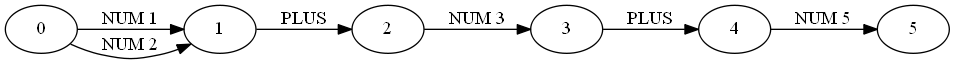
\includegraphics[width=150mm]{Pictures/Conflict.png}
\caption{Входной граф, содержащий Shift/Reduce конфликт.}
\label{shift_reduce_conflict}
\end{figure}

Для данного графа в результате синтаксического разбора будет построено целых четыре дерева разбора, т.к. для каждого пути будет построено по два дерева (ввиду неоднозначности грамматики). Однако порождённые конфликтом Shift/Reduce деревья соответствуют одному и тому же пути в графе, а значит, множества их листьев совпадают. Поэтому в данном примере при поддержке подсветки синтаксиса для каждого пути в графе достаточно рассмотреть только одно из таких деревьев. То же самое верно и для Reduce/Reduce конфликта. 

Наиболее сложной для реализации поддержки языков является, соответствующая ветвлению во входном графе. Сложность заключается в том, что в худшем случае для покрытия всех токенов придётся рассматривать все возможные деревья разбора. На рисунке \ref{bad_case} продемонстрирован пример такого входного графа. 

\begin{figure}[h]
\centering
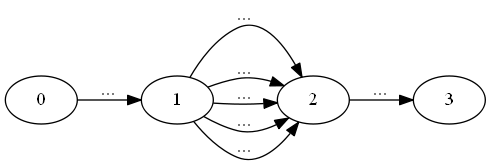
\includegraphics[width=100mm]{Pictures/Bad_case.png}
\caption{Входной граф, в котором необходимо рассмотреть все деревья разбора.}
\label{bad_case}
\end{figure}

Однако поскольку в вопросе подсветки деревьев скорость является одним из самых критичных, то принято решение осуществлять генерацию деревьев ленивым образом. Это позволит сэкономить время и память. 

Для того чтобы описать алгоритм извлечения деревьев из SPPF, введём следующие обозначения.
\begin{itemize}
\item OutEdges ($v$) ~-- количество исходящих дуг из вершины $v$. 
\item Succ ($v$) ~-- $\{u \mid \mbox{существует дуга из вершины } v \mbox{ в вершину u} \}$.
\item Tokens ($v$) ~-- количество токенов, которые принадлежат графу с корнем $v$.
\end{itemize}

На вход алгоритму подаётся граф разбора и множество $unprocessed$ - множество токенов, которые нужно посетить. $root$ = корень графа разбора. Все вершины окрашены в белый цвет. 

Вернуть GetTree (root, unprocessed).

GetTree (v, unprocessed):
\begin{itemize}
\item Если unprocessed = $\emptyset$, то вернуть пустое дерево (null).
\item Иначе вернуть Handle (v, unprocessed).
\end{itemize}

Handle (v, unprocessed):
\begin{enumerate}
\item Если вершина v - вершина-символ, то 
    \begin{itemize}
        \item Если OutEdges (v) == 0, то это значит, вершина $v$ соответствует какому-то токену $t$. unprocessed = unprocessed $\setminus \{t\}$; 
        \item Если OutEdges (v) == 1, то Handle (Succ (v), unprocessed).
        \item Если OutEdges (v) > 1, то 	$s = arg \; max_{u \in Succ(v)} \; \mid \mbox{Tokens (u)} \cap \mbox{unprocessed} \mid$. Handle (s, unprocessed). // т.е. идём по тому поддереву, которое содержит в себе наибольшее количество токенов из множества unprocessed. 
    \end{itemize}
    Перейти к шагу 3.
\item Если текущая вершина - вершина-продукция, то для каждой вершины $u \in$ ~Succ(v) сделать следующее:  Handle (u, unprocessed). Перейти к шагу 3.
\item Покрасить v в чёрный цвет. Если v == root, то перейти к шагу 4.
\item Алгоритм завершает работу. Вернуть дерево, состоящее из “чёрных” вершин, и множество unprocessed. 
\end{enumerate}

Рассмотрим работу алгоритма на примере входного графа, изображённого на рисунке ~\ref{illustration_input}.

\begin{figure}[h]
\centering
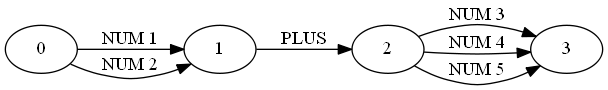
\includegraphics[width=100mm]{Pictures/Illustration.png}
\caption{Пример входного графа.}
\label{illustration_input}
\end{figure}

Граф разбора для такого входа будет выглядеть следующим так, как показано на рисунке ~\ref{illustration_sppf}.

\begin{figure}[h]
\centering
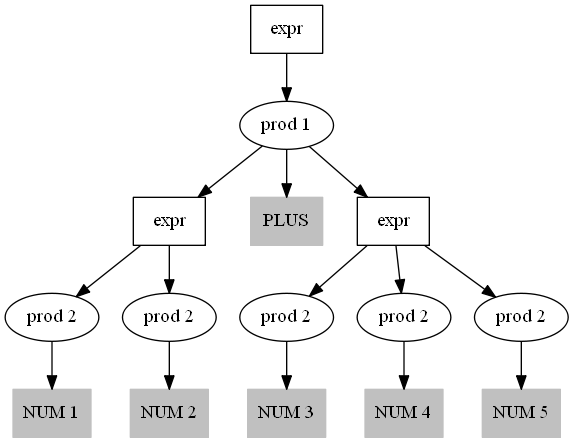
\includegraphics[height=70mm]{Pictures/Illustration_sppf.png}
\caption{SPPF для предыдущего примера.}
\label{illustration_sppf}
\end{figure}

При генерации первого дерева из этой структуры у нас все токены считаются непокрытыми. Поэтому алгоритм на вход принимает множество, состоящее из всех токенов. Поскольку любое из шести возможных деревьев разбора содержит три токена, то алгоритм вернёт любое из них. Предположим, что он вернул дерево, изображённое на рисунке ~\ref{Illustration_res1}. 

\begin{figure}[h]
    \centering
    \begin{subfigure}{0.25\textwidth}
        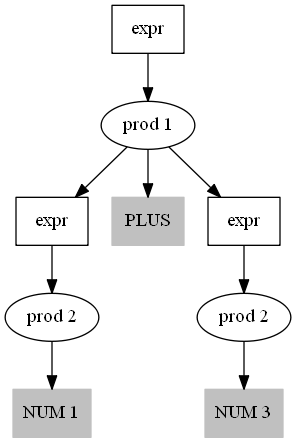
\includegraphics[height=70mm]{Pictures/Illustration_res1.png}
        \caption{Результат первого запуска алгоритма.}
        \label{Illustration_res1}
    \end{subfigure}
    \qquad
    \begin{subfigure}[h]{0.25\textwidth}
        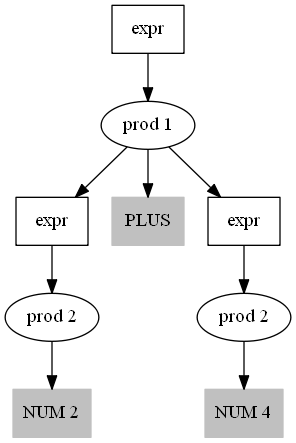
\includegraphics[height=70mm]{Pictures/Illustration_res2.png}
        \caption{Результат второго запуска алгоритма.}
        \label{Illustration_res2}
    \end{subfigure}
    \qquad
    \begin{subfigure}[h]{0.25\textwidth}
        \centering
        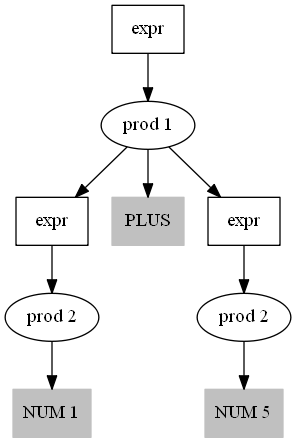
\includegraphics[height=70mm]{Pictures/Illustration_res3.png}
        \caption{Результат третьего запуска алгоритма.}
        \label{Illustration_res3}
    \end{subfigure}
    \caption{Деревья для графа на рисунке ~\ref{illustration_sppf}, которые покрывают все токены}
\end{figure}

Также вместе с этим деревом вернётся множество, состоящее из токенов NUM 2, NUM 4 и NUM 5. Это множество передаётся алгоритму при втором запуске. 

На основе этой информации алгоритм снова начинает обход графа с “корня”. На этот раз существует два дерева, которые содержат в себе два “новых” токена (т.е. токена из переданного на вход множества), три дерева, которые содержат в себе один “новый” токен, и одно дерево, которое не содержит в себе “новых” токенов (то, которое было возвращено при предыдущем запуске). Алгоритм выбирает одно из деревьев, которое содержит в себе наибольшее количество новых токенов (см. рисунок ~\ref{Illustration_res2}). Также возвращается множество, состоящее из NUM 5 - токен, который ещё не покрыли. 

При третьем запуске алгоритм на вход получает множество, состоящее из NUM 5, и снова начинает обход с корня. На этот раз существует четыре дерева, которые не содержат в себе новых токенов, и два дерева, которые содержат в себе один новый токен. И вернёт алгоритм вместе с одним из таких деревьев (например, как на рисунке ~\ref{Illustration_res3}) ещё и пустое множество. 

Если запустить алгоритм, передав ему на вход пустое множество, то он вернёт null, не начиная обхода. Это будет означать, что все возможные “листья” уже покрыты. 